% !TeX spellcheck = de_DE
\documentclass[
			   fontsize=11pt,
               paper=a4,
               bibliography=totoc,
               idxtotoc,
               headsepline,
               footsepline,
               footinclude=false,
               BCOR=12mm,
               DIV=13,
               openany,   % using this removes blank pages around part / chapter starts.
%               oneside    % include this if you have to print only one page per sheet of paper.
               ]
               {scrbook}

%%% SETTINGS

% no word wrapping
%\righthyphenmin=62
%\lefthyphenmin=62
% fewer hyphens
\usepackage{microtype}

% german symbols
\usepackage[utf8]{inputenc}

% strikethrough by \sout
\usepackage[normalem]{ulem}

% insert graphics
\usepackage{graphicx}
% more flexible figures e.g. graphics with captions beside them
\usepackage{floatrow}
% more flexible captions.
% Use \captionsetup{options} to configure,
% use it in an environment for local setup
\usepackage{caption}
% subfigures (see template):
\usepackage{subcaption}

% more control of enumerations and itemizations
\usepackage{enumitem}
% less space between items
\setlist[itemize]{itemsep=0cm}
\setlist[enumerate]{itemsep=0cm}
% more customizeable tables (e.g. multiple lines per cell)
\usepackage{tabularx}
% fix for vertical centering
\usepackage{ragged2e}
\renewcommand\tabularxcolumn[1]{>{\Centering}m{#1}}
% column types with multiple lines and formatting
\usepackage{array}
\newcolumntype{C}{>{\centering\arraybackslash}X}
\newcolumntype{R}{>{\raggedleft\arraybackslash}X}
\newcolumntype{L}{>{\raggedright\arraybackslash}X}
% merge multiple rows \multirow{2}{*}{bla} & \\ &
\usepackage{multirow}
% activate for tables with page breaking
%\usepackage{ltablex}
% fix for table movement and itemizations
%\keepXColumns

% fix for dynamics spaces after custom commands
\usepackage{xspace}

% tabbing: use with \tab
\usepackage{tabto}
\TabPositions{4cm}

%% fancy math
% propper matrices, underbrace text
%\usepackage{amsmath}
\usepackage{mathtools}
% special symbols e.g. squares
\usepackage{amssymb}

%% plotting
\usepackage{pgfplots}
\usepgfplotslibrary{fillbetween}

%%Settings for code
% code placement right there
\usepackage{float}
% code coloring
\usepackage{xcolor}
% code listing
\usepackage{listings}

% flexible multi column style
\usepackage{multicol}

% graphs
\usepackage{tikz}
\usetikzlibrary{shapes.geometric, arrows}
% define some elements
\tikzstyle{box} = [rectangle, rounded corners, minimum width=3cm, minimum height=1cm,text centered, draw=black, fill=black!5]
\tikzstyle{arrow} = [thick,->,>=stealth]
\usepackage{varwidth}

% Some code highlighting styles you can use with lstlistings
% C++ code style similar to default eclipse
\lstdefinestyle{eclipse-cpp} {
    captionpos=b,
    language=C++,
    otherkeywords={final},
    basicstyle=\footnotesize,
    numbers=left,
    numberstyle=\small,
    showstringspaces=false,
    tabsize=2,
    frame=single,
    breaklines=true,
    keywordstyle=\bfseries\color[RGB]{127,0,85},
    identifierstyle=\color[RGB]{0,0,192},
    stringstyle=\color[RGB]{42,0,255},
    commentstyle=\color[RGB]{63,127,95},
}

% If no highlighting is intended
\lstdefinestyle{plain}{
	basicstyle=\ttfamily\footnotesize,
}

\lstdefinestyle{cmd}
{
	basicstyle=\ttfamily\footnotesize,
	captionpos=b,
	language=bash,
	otherkeywords={final},
	numbers=left,
	numberstyle=\small,
	showstringspaces=false,
	frame=single,
	breaklines=true,
}

% fancy algorithms (see template)
\usepackage[ruled, vlined, linesnumbered]{algorithm2e}
\DontPrintSemicolon
\SetKw{KwBy}{by}
\SetKw{KwAnd}{and}

% clickable links and clickable table of content <3
% Options: links with linebreaks
\PassOptionsToPackage{hyphens}{url}
\usepackage[bookmarks=false]{hyperref}
\hypersetup{
    colorlinks,
    citecolor=black,
    filecolor=black,
    linkcolor=black,
    urlcolor=black
}
% Alterations to labels used by \autoref{}: Capitalize everyything
\def\chapterautorefname{Chapter}
\def\sectionautorefname{Section}
\def\subsectionautorefname{Subsection}
\def\algorithmautorefname{Algorithm}
\def\subfigureautorefname{Figure}
% for custon stuff like use:
% \hyperref[custom:foo]{Custom~\ref*{custom:foo}}

% -------------------------------------------------------------------------------
% ------------------------- Bibliography Customisation ------------------------
% -------------------------------------------------------------------------------

% replace \makebibliography with this package to enable nice formatting for citing web pages
\usepackage[%
backend=bibtex				% biber or bibtex
,style=numeric-comp		% numerical-compressed TODO: Check if plain is fine as style (was 'alpha' before I changed it)
,sortcites=true				  % sorts citations if multiple entry keys are passed to a citation command
,isbn=true
,url=true
,doi=true
%,natbib=true         % if you need natbib functions
]{biblatex}
\addbibresource{literature.bib}  % better than \bibliography
\usepackage{lipsum} % for filling pages with stuff

% -------------------------------------------------------------------------------
% -------------------------- Glosssary Customisation --------------------------
% -------------------------------------------------------------------------------
% For some reason this did not work when located in settings.tex
% Any links in resulting glossary will not be "clickable" unless you load the glossaries package after the hyperref package.

\usepackage{xparse}
\usepackage[acronym,toc]{glossaries}

\DeclareDocumentCommand{\newdualentry}{O{}D<>{}m m m m m } {
	\newglossaryentry{gls-#3}{
		name={#5},
		text={#5\glsadd{gls-#3}},
		description={#6},
		plural={#7},
		#1
	}
	\newacronym[see={[Glossary:]{gls-#3}},#2]{#3}{#4}{#5\glsadd{gls-#3}}
}

% use the \newdualentry command like this:
% \newdualentry{OWD}    																			% label
% 	{OWD}		            																				 % abbreviation
% 	{One-Way Delay} 	   																				% long form
% 	{The time a packet uses through a network from one host to another}	  % description
%   {OWDs}																							   % abbreviation in plural

\makeglossaries
% -------------------------------------------------------------------------------
% ---------------------- Acronyms and Glossary Definition ---------------------
% -------------------------------------------------------------------------------

\newacronym{nnapi}{NNAPI}{Neural Networks API}

\newacronym{cv}{CV}{Computer Vision}

\newacronym{cnn}{CNN}{Convolutional Neural Network}

\newacronym{resnet}{ResNet}{Residual Neural Network}

\newacronym{relu}{ReLU}{Rectified Linear Unit}

\newacronym{ml}{ML}{Machine Learning}

\newacronym{ann}{ANN}{Artificial Neural Network}
	
\newdualentry{api} %oxford dictionary
	{API}
	{application programming interface}
	{set of functions and procedures allowing the creation of applications that access the features or data of an operating system, application, or other service}
	{APIs}

\newglossaryentry{diff_privacy} %https://oconnell.fas.harvard.edu/files/salil/files/differential_privacy_primer_nontechnical_audience.pdf
{
	name={differential privacy},
	description={protects an individual’s information essentially as if her information were not used in the analysis at all, in the sense that the outcome of a differentially private algorithm is approximately the same whether the individual’s information was used or not}
}

% -------------------------------------------------------------------------------
% --------------------------------- Thesis Info ---------------------------------
% -------------------------------------------------------------------------------

% set title, authors and stuff for the cover
% docytype needs xspace because it is used within text.
\def\doctype{Bachelor's Thesis\xspace}

\def\studyProgram{Informatics}
\def\title{Implementing a mobile app for object detection}

\def\titleGer{Entwicklung einer mobilen App zur Objekterkennung}
\def\author{David Drews}
% Prof
\def\supervisor{Univ.-Prof. Dr. Hans-Joachim Bungartz}
% PhD Candidate
\def\advisor{Severin Reiz, M.Sc.}
\def\date{15th of August 2021}

\begin{document}
\frontmatter
% -------------------------------------------------------------------------------
% ---------------------------------- COVERPAGE ------------------------------
% -------------------------------------------------------------------------------

% correct BCOR - undo at the end !!!
\def\bcorcor{0.15cm}
\addtolength{\hoffset}{\bcorcor}
\thispagestyle{empty}
\vspace{4cm}
\begin{center}
    
\includegraphics[width=4cm]{templateStuff/tumlogo.pdf}\\[5mm]
    \huge DEPARTMENT OF INFORMATICS\\[5mm]
    \large TECHNICAL UNIVERSITY OF MUNICH\\[24mm]

    {\Large \doctype in \studyProgram}\\[20mm]
    {\huge\bf \title\par}
    \vspace{15mm}
    {\LARGE  \author}
    \vspace{10mm}
    \begin{figure}[h!]
        \centering
        
\includegraphics[width=4cm]{templateStuff/informat.pdf}
   \end{figure}
\end{center}

\cleardoubleemptypage

% -------------------------------------------------------------------------------
% ---------------------------------- TITLEPAGE --------------------------------
% -------------------------------------------------------------------------------

\def\bcorcor{0.15cm}
\addtolength{\hoffset}{\bcorcor}
\thispagestyle{empty}
\vspace{10mm}
\begin{center}
    
\includegraphics[width=4cm]{templateStuff/tumlogo.pdf}\\[5mm]
	\huge DEPARTMENT OF INFORMATICS\\[5mm]
	\large TECHNICAL UNIVERSITY OF MUNICH\\[24mm]
	{\Large \doctype in \studyProgram}\\[20mm]
	{\LARGE\textbf \title}\\[10mm]
	{\LARGE\textbf \titleGer}\\[10mm]
	\begin{tabular}{ll}
		\Large Author:      	& \Large \author \\[2mm]
		\Large Supervisor:  	& \Large \supervisor\\[2mm]
		\Large Advisor:			& \Large \advisor\\[2mm]
		\Large Submission Date:       		& \Large \date
	\end{tabular}
	\vspace{-1mm}
	\begin{figure}[h!]
		\centering
		
\includegraphics[width=4cm]{templateStuff/informat.pdf}
	\end{figure}
\end{center}

% undo BCOR correction
\addtolength{\hoffset}{\bcorcor}
\newpage

% -------------------------------------------------------------------------------
% ---------------------------------- DISCLAIMER -------------------------------
% -------------------------------------------------------------------------------

\cleardoubleemptypage

\thispagestyle{empty}
\vspace*{0.7\textheight}
\noindent
I confirm that this \MakeLowercase{\doctype} is my own work and I have documented all sources and material used.\\

\vspace{15mm}
\noindent
Munich, \date \hspace{5cm} \author
\cleardoubleemptypage

% -------------------------------------------------------------------------------
% ---------------------------------- ABSTRACT --------------------------------
% -------------------------------------------------------------------------------

\phantomsection
\addcontentsline{toc}{chapter}{Abstract}
\vspace*{2cm}
\begin{center}
    {\Large \textbf {Abstract}}
\end{center}
\vspace{1cm}

\lipsum[2]

\cleardoublepage

% -------------------------------------------------------------------------------
% ------------------------------ TABLE OF CONTENTS -------------------------
% -------------------------------------------------------------------------------

\tableofcontents
\thispagestyle{empty}
\cleardoubleemptypage

% -------------------------------------------------------------------------------
% --------------------------------- MAIN MATTER ------------------------------
% -------------------------------------------------------------------------------

\mainmatter
\chapter{Motivation}

The aim of this work was to further develop the Android app TUM-Lens \cite{lensApp}. The core functions of the app include the analysis of images that are captured via the camera of the Android device and transmitted to the app as a live feed. For an optimal user experience, the analysis of the images must take place in near real time. This is the only way to ensure that the analysis results displayed always match the current content of the camera feed, which can change very quickly due to panning of the camera by its user. While in many applications the analysis of image data can take place decentrally in powerful data centres, in the case of TUM-Lens the image analysis runs on the mobile device itself. With the completion of this work, image analysis now also includes object detection in addition to the classification of images.

%\section{Increasing Computation Power on Mobile Devices} %TODO: will probably not elaborate here as 3 topics for motivation might be enough

\section{Growing Support for Running Machine Learning Operations on Mobile Platforms}

Support for the development of \gls{ml} and also in particular deep learning applications for smartphones is growing steadily and from different directions at the same time. Developer-friendly frameworks such as TensorFlow, developed by Google Brain, or PyTorch, developed by Facebook's AI Research Lab, are among the best-known deep learning frameworks~\cite{dl_ranking_2018}. The release of TensorFlow Lite\footnote{\url{https://www.tensorflow.org/lite}} 2017~\cite{tflite_release_verge_2017} and PyTorch Mobile 2019~\cite{pytorch_release_2019} show that mobile platforms increasingly come into focus of companies providing \acrlong{ml} software. In recent year, device manufacturers and operating system developers also started to provide dedicated hardware and software components for mobile machine learning. Examples include Apple's Neural Engine~\cite{neural_engine_verge_2017}, unveiled in 2017, or Android's \gls{nnapi}~\cite{nnapi_devguide_2021}. Apple's Neural Engine is a hardware component optimised for \acrlong{ml} requirements. Android's \gls{nnapi}, on the other hand, is an Android C \gls{api} for efficient computation of \gls{ml} operations and provides a basic set of functions for higher-level \gls{ml} frameworks. As a result of these developments, it is becoming easier for developers to build \gls{ml} applications that run efficiently on mobile devices. This support was a major catalyst for the initial and further development of TUM-Lens in the context of two bachelor theses.

\section{Offline Usability}

TUM-Lens is more independent compared to many other \acrlong{ml} based apps as it does not require an internet connection to use it. Often, apps and services by definition need a connection to the internet to perform their task. The Amazon voice assistant Alexa can answer simple voice commands to control smart home devices or check the time without an internet connection and thus already uses on-device \acrlong{ml}. But even if Alexa could analyse and understand all voice commands locally, the request would still have to be forwarded to the Amazon servers in most cases. Due to the large number of possible queries, not all answers can be kept on the device, but must be retrieved from the Internet. Such queries include daily topics such as the weather report, traffic or the result of a sporting event. However, an internet connection is not required to use the full range of functions of TUM-Lens. All the information needed for image classfification and object detection is stored locally on the device in the form of various already trained \gls{ann}. With the integration of the corresponding mobile frameworks, the image analysis can therefore be carried out locally on the device, making the app independent of an internet connection.

\section{Improved Privacy}

The use of on-device \gls{ml} provides another mechanism for protecting personal data in the context of machine learning in addition to existing methods such as \gls{diff_privacy}. Due to the growing support for mobile \gls{ml} applications mentioned above, but also due to the independently increasing power of mobile devices~\cite{mobile_cpu_power}, not only the use of pre-trained \glspl{ann} becomes possible, but also the training of new \glspl{ann} on the mobile device itself becomes more and more relevant~\cite{liu19}. If the training process takes place locally on the device itself, no data needs to be transferred to external instances such as a company's servers. This makes it possible to develop applications that adapt more and more individually to the user as they are used, while guaranteeing maximum data protection. An example of the development of such an application is DeepType~\cite{deepType}. DeepType attempts to predict the next word used when the user enters the keyboard. While every user initially starts with the same pre-trained version of the \gls{ann} used by DeepType, the application continues to train this \gls{ann} with each input and thus adapts more and more to the characteristic input behaviour of the user without the text inputs ever leaving the device.

\chapter{Background Theory}

\section{Important Concepts}

Everybody is talking about \acrfull{ml}. It is already impossible to imagine our everyday life without the use of the term. Due to the multitude of contexts in which \acrfull{ml} is spoken of, some justifiably and some unjustifiably, it is important to create a common understanding for the theoretical content of this work.

%TODO: Maybe outline the different concepts that will be explained as their connection is loser than the other parts of the thesis.

\subsection{Machine Learning}

A popular definition of \gls{ml} is attributed to Arthur Samuel describing it as the "field of study that gives computers the ability to learn without being explicitly programmed"\footnote{Althought cited in popular machine learning material like Andrew Ng's \gls{ml} course at Stanford~\cite{mlCourseStan} the quote appears neither in Samuel's 1959~\cite{mlQuote1959} nor his 1967 paper~\cite{mlQuote1967}.}. \acrlong{ml} algorithms circumvent this need for explicit programming by improving an internal model through data. This process is called training and the data used to train the model is often regarded to as the model's experience~\cite{mlMitchell}. As depicted in figure \ref{fig:mlClassification}, \gls{ml} can be divided into the subfields supervised learning, unsupervised learning, semi-supervised learning and reinforcement learning.

\begin{figure}[H]
	\centering
	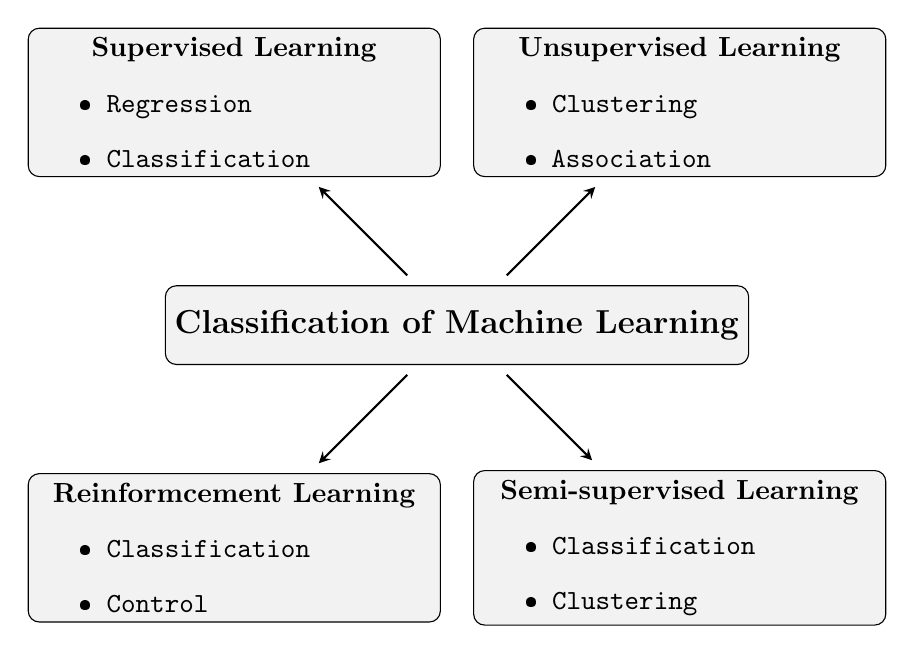
\begin{tikzpicture}[node distance=4cm]
		\node[box] (ml) {\large{\textbf{Classification of Machine Learning}}};
		\node[box, above left of = ml] (supervised) {
			\begin{minipage}{5cm}
				\centering\textbf{Supervised Learning}
				\begin{itemize}
					\item \texttt{Regression}
					\item \texttt{Classification}
				\end{itemize}
			\end{minipage}
		};
		\node[box, above right of = ml] (unsupervised) {
			\begin{minipage}{5cm}
				\centering\textbf{Unsupervised Learning}
				\begin{itemize}
					\item \texttt{Clustering}
					\item \texttt{Association}
				\end{itemize}
			\end{minipage}
		};
		\node[box,  below right of = ml] (semisupervised) {
			\begin{minipage}{5cm}
				\centering\textbf{Semi-supervised Learning}
				\begin{itemize}
					\item \texttt{Classification}
					\item \texttt{Clustering}
				\end{itemize}
			\end{minipage}
		};

		\node[box, below left of = ml] (reinforcement) {
			\begin{minipage}{5cm}
				\centering\textbf{Reinformcement Learning}
				\begin{itemize}
					\item \texttt{Classification}
					\item \texttt{Control}
				\end{itemize}
			\end{minipage}
		};
		\draw[arrow, shorten >= 5pt, shorten <= 5pt] (ml) -- (supervised);
		\draw[arrow, shorten >= 5pt, shorten <= 5pt] (ml) -- (unsupervised);
		\draw[arrow, shorten >= 5pt, shorten <= 5pt] (ml) -- (semisupervised);
		\draw[arrow, shorten >= 5pt, shorten <= 5pt] (ml) -- (reinforcement);
	\end{tikzpicture}
	\caption[Classification of Machine Learning]{The field of \acrlong{ml} divided into subfields by the characteristics of the underlying learning process. Also indicates the learning problems that are typically tried to be solved by applying the respective learning process.}
	\label{fig:mlClassification}
\end{figure}

\subsubsection{Supervised Learning}
In supervised learning, the learning machine is provided with input data as well as the output that is expected for the given input~\cite{introSupervised}. In the classical case of spam filtering, the input can be a collection of emails and the expected output is a label attached to each email that either classifies it as spam or as non-spam. The learning machine is then fed all e-mails as input data and learns to recognise which information in the input is important to produce the correct classification. As the system knows the correct answer for each training input, it can process an email, predict whether or not it is spam, and then use the known answer to change its weights in a way that will make it more likely to lead to a correct prediction and less likely to lead to a false prediction the next time it is presented with similar input.

\subsubsection{Unsupervised Learning}
Detecting hidden patterns and structuring data is where unsupervised learning comes into play. Learners of this type don't need to be provided with an expected output while being trained~\cite{introUnsupervised}. A scenario for the application of unsupervised learning is the problem of dividing a customer base into subgroups in order to treat every subgroup according to their specific needs. An employee might help the machine learning system by providing the number of subgroups she wants the system to generate. The learner then builds up its representation of the internal structure of the entire data set with every input it processes. After having processed enough customers, it will most likely have identified the key metrics that distinguish customers into the different groups. 

\subsubsection{Semi-Supervised Learning}
One use for semi-supervised learning is cluster analysis, which was already used as an example in the previous paragraph. In the case of semi-supervised learning, the system no longer has to work out the different groups (also known as \textit{clusters}) from the unlabelled data alone. Instead, it can use a small set of already labelled customers as a reference and build its internal representation of the entire dataset (labelled and unlabelled) around the clusters indicated by the pre-labelled data. This is especially useful because in many domains collecting or creating labelled data is difficult, expensive, or both~\cite{introSemiSup}.

\subsubsection{Reinforcement Learning}

Reinforcement learning is "learning what to do - how to map situations to actions - so as to maximize a numerical reward signal"~\cite{introRL}. Systems are trained via reinforcement learning to learn how to behave in dynamic environments. The tasks in these environments can stretch from playing a video game~\cite{rlStarCraft} to driving an autonomous car~\cite{rlCars}. These exemplary tasks show two characteristics that distinguish reinforcement learning from the other subfields of \gls{ml}: The reward signal is often delayed and attribution to single actions is difficult. Only once a game is won or the car has arrived safely at its destination the system knows if all the decisions it made along the way lead to a positive outcome. \textit{Trial-and-error} is therefore a term that summarises this learning paradigm quite precisely.


\subsection{Artificial Neural Networks}

An \acrlong{ann} - often just referred to as neural network - is a data processing concept that is inspired by biological neurons and their interconnectivity. As figures \ref{fig:2layeredANN} and \ref{fig:3layeredANN} show the artificial neurons (also called \textit{nodes}) in an \gls{ann} are grouped in \textit{layers}. There are three important types of layers: The \textit{input layer}\footnote{Note that the input layer is not counted towards the total number of layers in an \gls{ann}.}, the \textit{output layer} and an arbitrary number of \textit{hidden layers} in between the input and output layer. Similar to neurons in human brains, nodes of different layers can be connected. In \glspl{ann}, the nodes exchange signals in the form of numbers. Each node outputs a number that is computed by applying a non-linear function to its inputs. The output signal can then be a new input for other nodes or it can be part of the result returned by the output layer. The connections between nodes are also known as \textit{edges} and typically carry a weight. In the case of \glspl{ann}, the training process that is typical for all machine learning systems is the adjustment of these connection weights. The weights and other variables of the \gls{ann} are grouped under the term \textit{parameters}. In summary, an \gls{ann} transforms an input vector into an output vector through a series of non-linear functions, where both the calculation of the output and the training process are characterised by the specific structure of the \gls{ann} and its parameters.

%TODO: Maybe introduce a view typical ANN architectures like feed forward, convolutional, recurring, etc.

\subsection{Deep Learning}

Deep learning is a subarea of machine learning. Deep learning is characterised by the use of \glspl{ann} with many hidden layers. The more hidden layers a network has, the deeper it is. The deeper a network is and the more nodes the network has per layer, the more complex the computations that the \gls{ann} can successfully perform~\cite{dlBookGoodf}. As the number of layers and nodes grows, so does the number of parameters. Their large number is the reason deep learning requires extensive amounts of data to provide adequate results compared to other sub-disciplines of machine learning. Networks of this genus have been given the ability to perform extraordinarily complex computations at the expense of a resource-intensive training process.

\begin{multicols}{2} % defines an environment with two columns
	\begin{figure}[H] % [H] for EXACTLY HERE
		\centering
		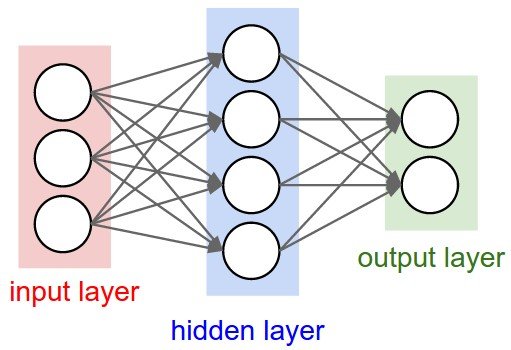
\includegraphics[height=3cm]{figures/ann1.jpeg}
		\caption[2-Layered ANN]{2-layered \gls{ann}. It is called fully connected as every node from the previous layer is connected to every node in the next layer. \\
			\tiny{Source:~\cite{annGraphics}}}
		\label{fig:2layeredANN} % labels always have to be placed after the caption
	\end{figure}
	
	\columnbreak    % start next column
	
	\begin{figure}[H] % [H] for EXACTLY HERE
		\centering
		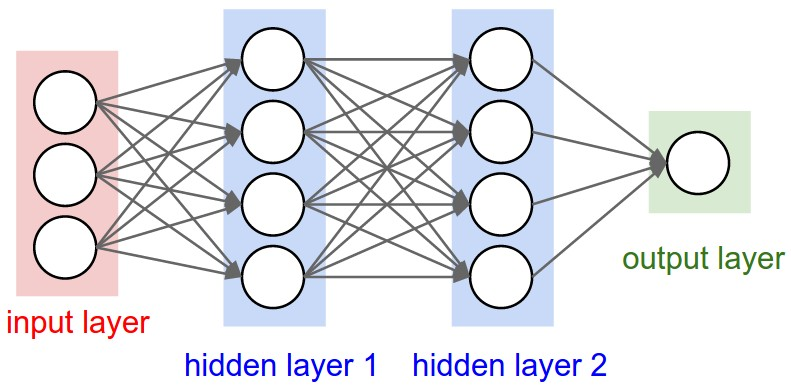
\includegraphics[height=3cm]{figures/ann2.jpeg}
		\caption[3-Layered ANN]{3-layered \gls{ann}. In \glspl{ann}, nodes in one layer are connected to nodes in other layers but not to other nodes in the same layer. \\
			\tiny{Source:~\cite{annGraphics}}}
		\label{fig:3layeredANN} % labels always have to be placed after the caption
	\end{figure}
\end{multicols}

\section{A Core Task of Computer Vision: Object Detection}



\subsection{How Object Detection Differs From Related Tasks}

The field of \gls{cv} encompasses numerous distinct problems and an even larger number of potential solutions. In the following, object detection as a typical task in the \gls{cv} context is distinguished from other \gls{cv} tasks that are closest to it in terms of learning objectives.

\begin{figure}[H] % [H] for HERE
	\centering
	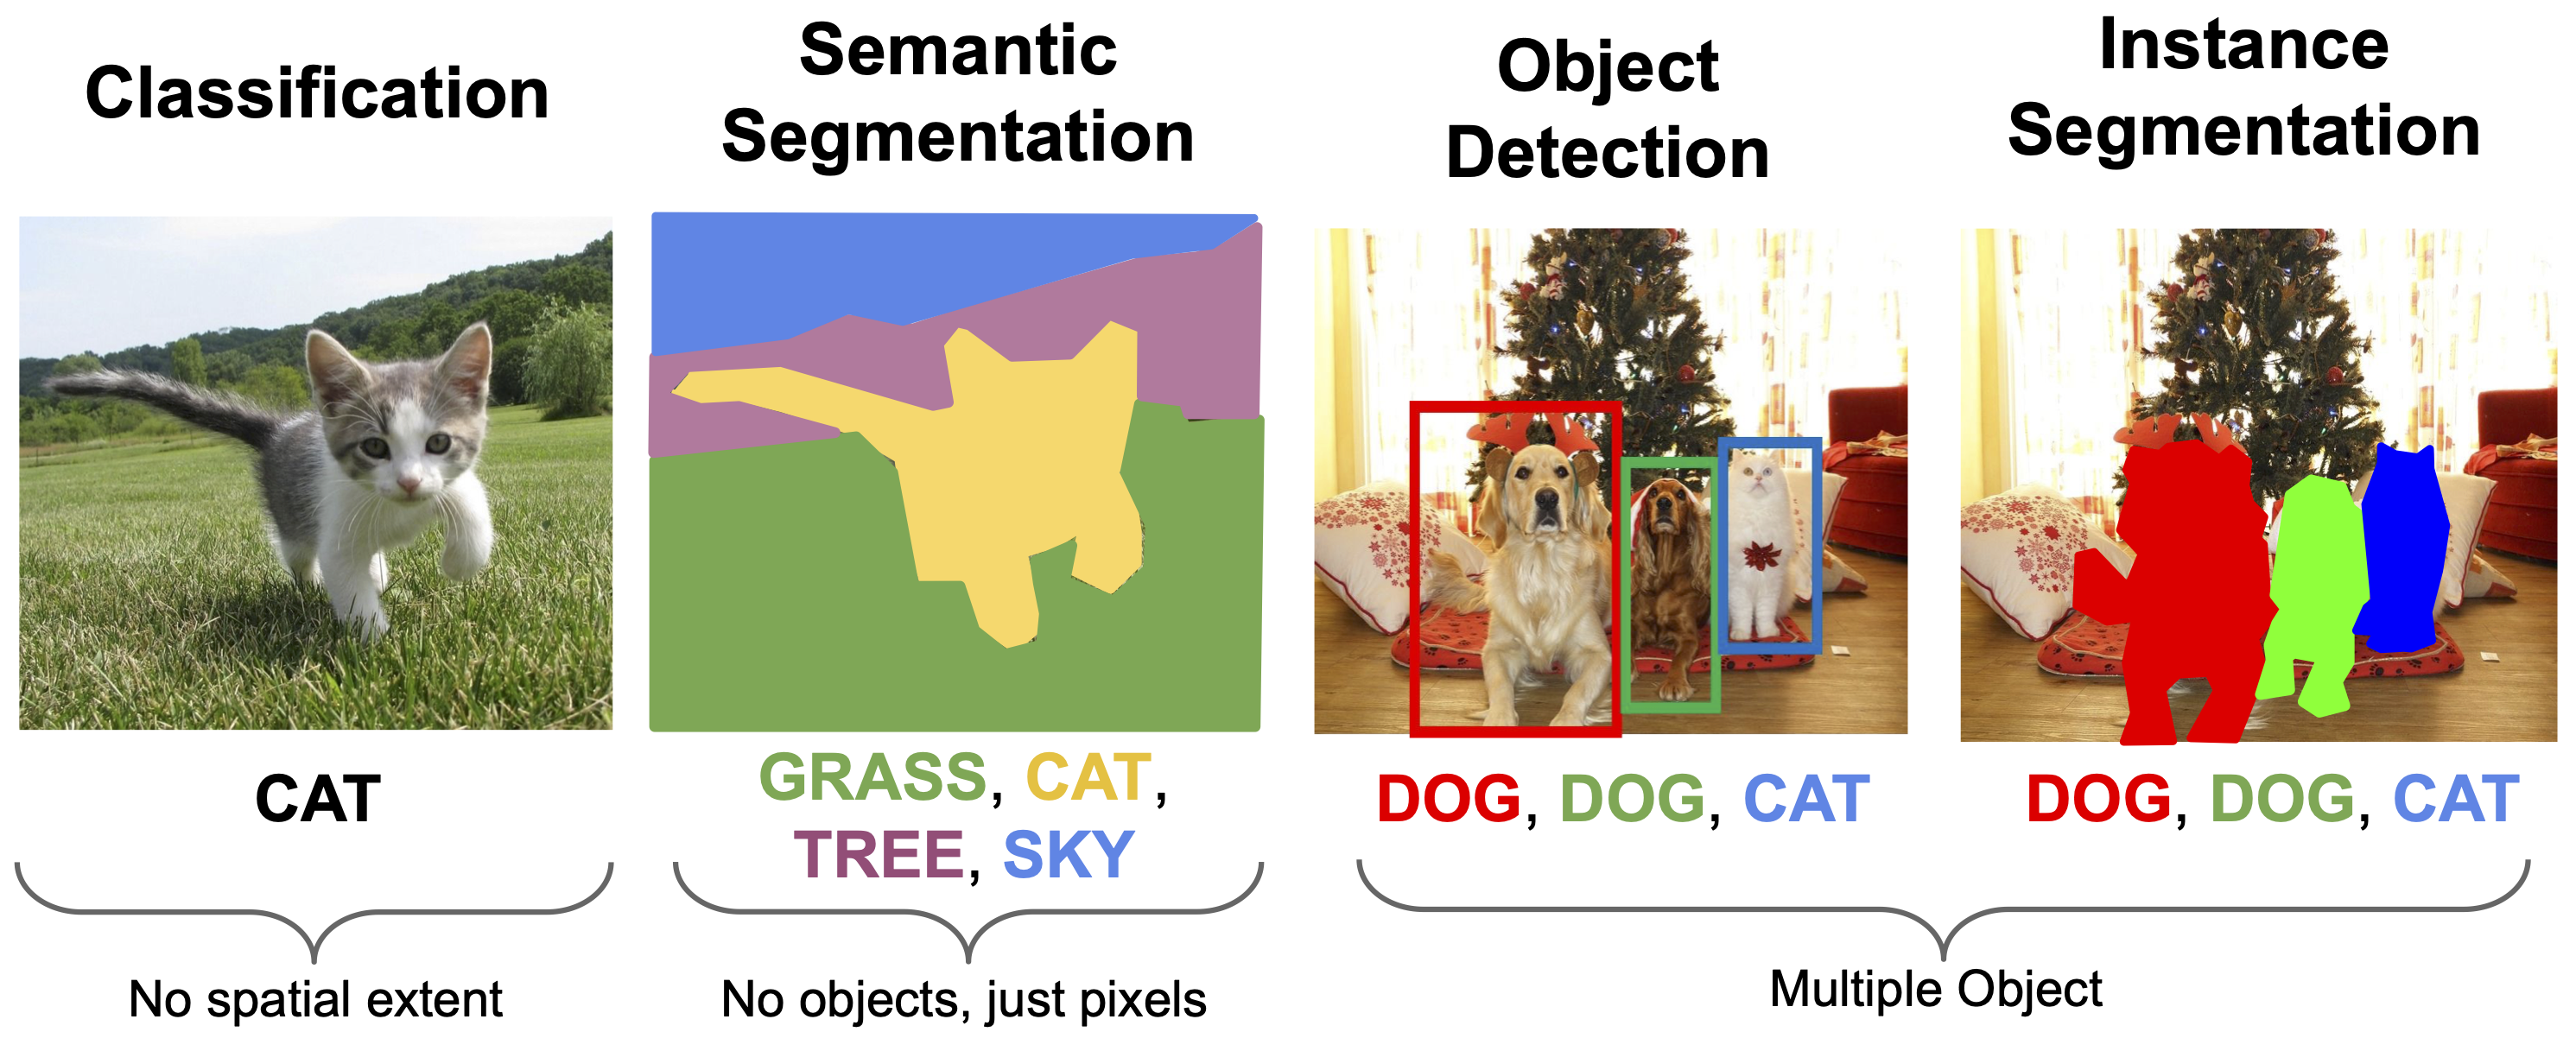
\includegraphics[width=\textwidth]{figures/detection_related_tasks.png}
	\caption[Typical Computer Vision Tasks]{Object detection differs conceptually from other related \gls{cv} tasks regarding spatial information, the concept of objects and the number of detections in a scene.\\
		\tiny{Source:~\cite{cvTasks}}}
	\label{fig:cvTasks} % labels always have to be placed after the caption
\end{figure}

\subsubsection{Semantic Segmentation}
In semantic segmentation, each pixel of an image is assigned a class. However, there are no objects. This means that if there are several objects of the same class in the image, all the associated pixels receive the same class label. Therefore, the different objects cannot be differentiated based on the result of the semantic segmentation.

\subsubsection{Image Classification}
In image classification, the result of the detection is a single class. In rare application variants, a bounding box for one object of the detected class is also returned - as a rule, however, no spatial extent is associated with the task of classification.

\subsubsection{Object Detection}
Object detection deals with the identification of any number of objects within an image. For each object, a class label and its position are returned as the coordinates of a rectangle enclosing the object. It is important here that, as depicted in Figure \ref{fig:cvTasks}, several objects of the same class can also be recognised. In contrast to the  task of semantic segmentation, the different objects of the same class can be distinguished.

\subsubsection{Instance Segmentation}
The instance segmentation essentially fulfils a better variant of the object detection. Again, several objects of different classes are detected and the positions of the classes are also part of the output. However, the positions are not marked by bounding boxes as in object detection, but each pixel belonging to an object receives a label of this object. The objects are therefore even more sharply separated from the image areas that do not contain an object and, in contrast to semantic segmentation, individual objects of the same class remain distinguishable.

%\section{Computer Vision on Mobile Devices}

\subsection{Architectures}

State of the art object detection algorithms run predominantly on deep learning architectures~\cite{dlForDetection}. The bachelor's thesis preceeding this work, \textit{Implementing a TensorFlow-Slim based Android app for image classification}~\cite{maxJokel}, already explains why \glspl{cnn} is the most widespread class of deep neural networks used for perceptual tasks. This explanation will therefore not be pursued here once more. Instead, we survey a selection of modern 

\subsubsection{R-CNN}

2014
\cite{rcnnIntro}



%Heute Spielarten wie Fast R-CNN, Faster R-CNN, Mask R-CNN

\subsubsection{MobileNet}

2017

%In der Implementierung verwendet

\subsubsection{RetinaNet}

2018


\subsubsection{CenterNet}

2019

\subsubsection{EfficientDet}

2019

%YOLO
%ShuffleNet 2018
%FBNet 2019

\subsection{MobileNetSSDv2: A Single Shot MultiBox Detector}

\subsubsection{Introduction to XYZ Networks}


\subsubsection{Some Deep}
\subsubsection{Dive Into}
\subsubsection{Object Detection}
\subsubsection{Theory Fun}

\chapter{App Development}

\section{Previous State of the Application}

\subsection{Use Cases}

\subsection{Notable Design Decisions}

\section{Development Goals}

\subsection{Migration From Java to Kotlin}

\subsection{New Functionality: Object Detection}

\section{Implementing Object Detection Based on the TensorFlow Lite Framework}

\subsection{Some Deep}
\subsection{Dive Into}
\subsection{Object Detection}
\subsection{Implementation Fun}

\subsection{Next steps in the development of TUM-Lens}

% Potential Contets: Design and architecture choices, reused patterns from exisiting application, improvements to exisiting code

\chapter{Results}

\section{Performance Evaluation}

\section{Accuracy}

\section{Possible Applications} % Can also be named "Future Work" depending on the contents of this section

Die Anwendungsbereiche von Computer Vision sind zahlreich. Zu den regelmäßigen Aufgaben im Bereich 

Organisation von Fotos auf dem Smartphone, ohne dass diese an die Server von Apple, \& Google Co geschickt werden müssen (Gruppieren von Fotos, die zu einem Urlaub gehören, Gesichtserkennung, Objekterkennung)

Autonome Autos werden unahängig von einer Verbindung zum Internet (5G, shared medium, bleibt das Auto im Tunnel dann stehen?)




% -------------------------------------------------------------------------------
% ----------------------------------- APPENDIX --------------------------------
% -------------------------------------------------------------------------------

\appendix

\chapter{Screenshots of the Application}

\chapter{Tips With Greetings From the Chair}
\label{sec:tips}       % labels can be put almost anywhere and can be referencef from anywhere.
Here are tips along the way:

\section{Tips}
\subsection{How to Describe}
% optional: set the spacing between columns
\setlength{\columnsep}{30 pt}
When listing several points you have three basic options:
\begin{multicols}{3}
	\begin{itemize}
		\item itemize
		\item enumerate
		\item description
	\end{itemize}
	
	\vfill\null
	\columnbreak
	
	\begin{enumerate}
		\item itemize
		\item enumerate
		\item description
	\end{enumerate}
	
	\vfill\null
	\columnbreak
	
	\begin{description}
		\item[itemize] short, unordered
		\item[enumerate] short ordered
		\item[description] listing of descriptions. Also nice for longer ones.
	\end{description}
	
\end{multicols}


\subsection{How to Quote}

\begin{quote}
	"This is a quote!"
\end{quote}

\begin{itemize}
	\item Citations to a source can be made like this \verb|\cite{gratl17task}| =~\cite{gratl17task}
	\subitem Always join text and the citation with a non-breaking space: \verb|text~\cite{foo}|.
	\item Referencing Sections, Figures, Tables, Formulas: \verb|\autoref{sec:tips}| = \autoref{sec:tips}.
	\item Footnotes for url or further notes: \verb|\footnote{\url{https://www.top500.org}}| = \footnote{\url{https://www.top500.org}}
\end{itemize}

\subsection{How to Math}

Use the align environment for equations especially if you want to align them somehow.

\begin{align}
	1 + 1 &\ne 3\\
	\left(\dfrac{10}{1}\right) - 9 &= 1
\end{align}

% if you need a pagebreak because figure placement is broken:
\clearpage

\section{Environments}

\subsection{How to Figure}

Anything can also be put in multiple columns.

\begin{multicols}{2} % defines an environment with two columns
	\begin{figure}[H] % [H] for HERE
		\centering
		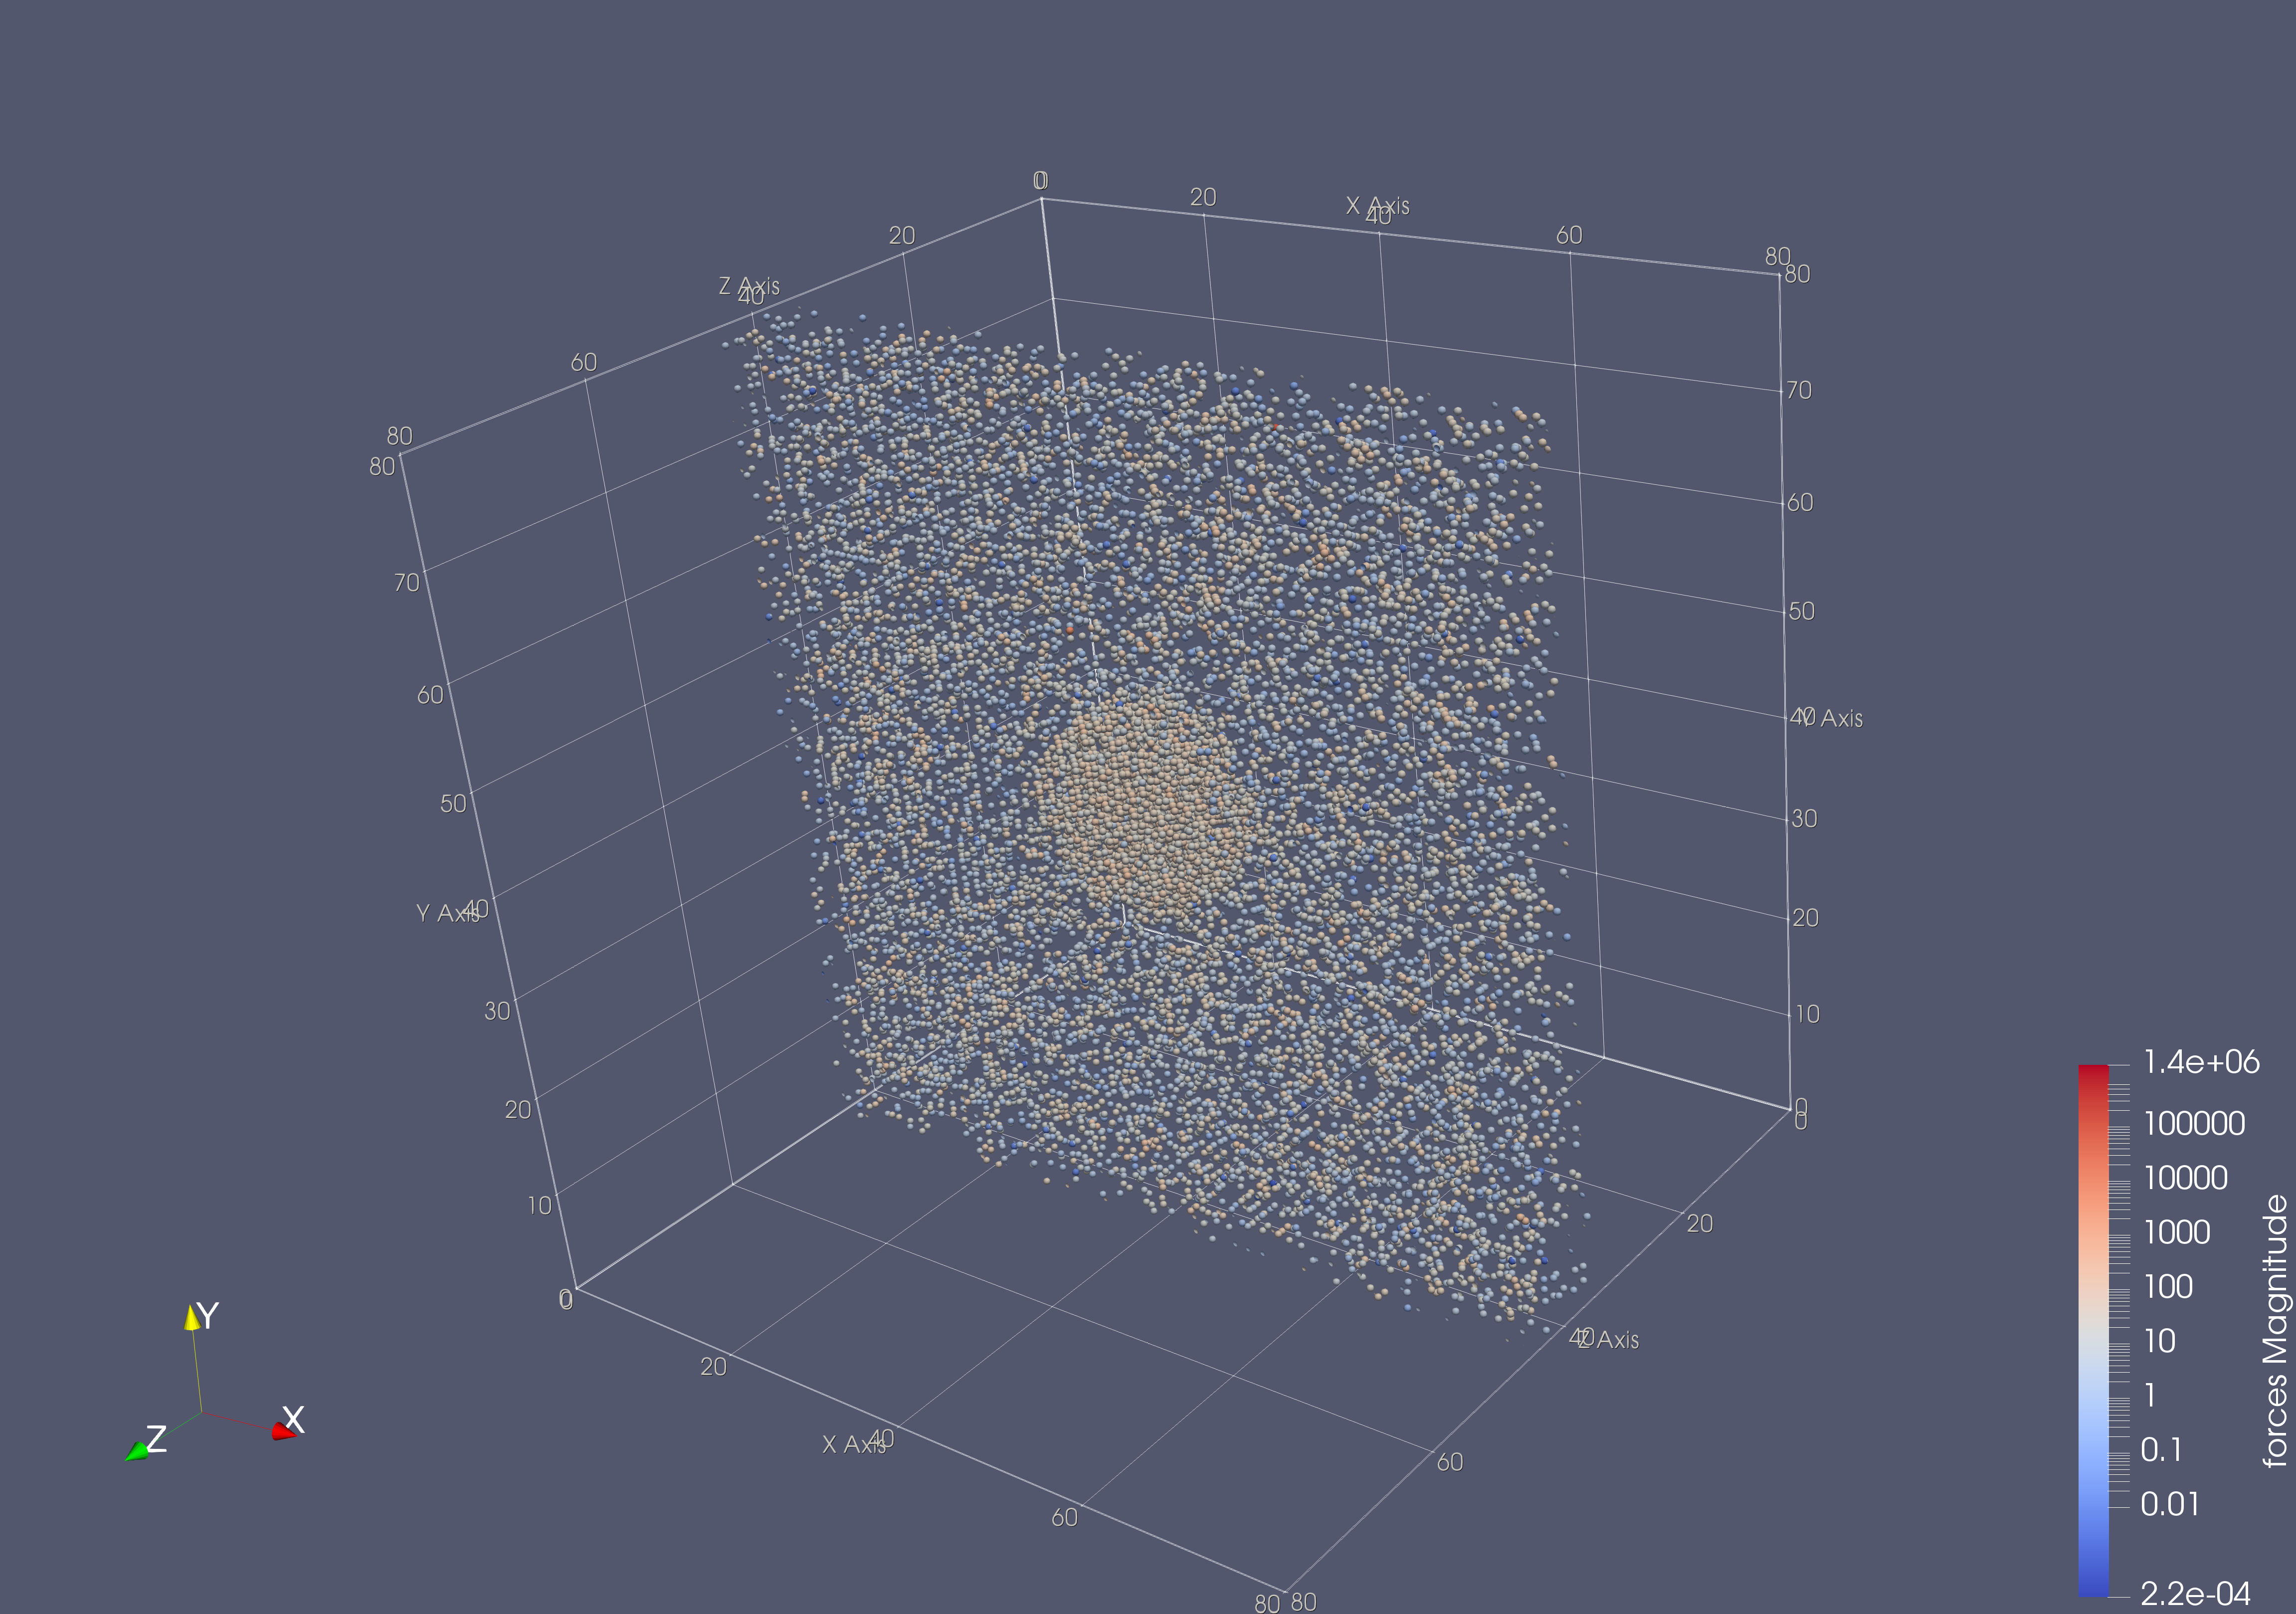
\includegraphics[width=.9\columnwidth]{figures/scenario_clip_rot.png}
		\caption[Example Figure]{Some Caption. Always also include a source if it wasn't created by you!\\
			\tiny{Source:~\cite{gratl17task}}}
		\label{fig:exampleLabel1} % labels always have to be placed after the caption
	\end{figure}
	
	\columnbreak    % start next column
	
	\begin{figure}[H]
		\centering
		\begin{tikzpicture}
			\node[anchor=south west,inner sep=0] (image) at (0,0) {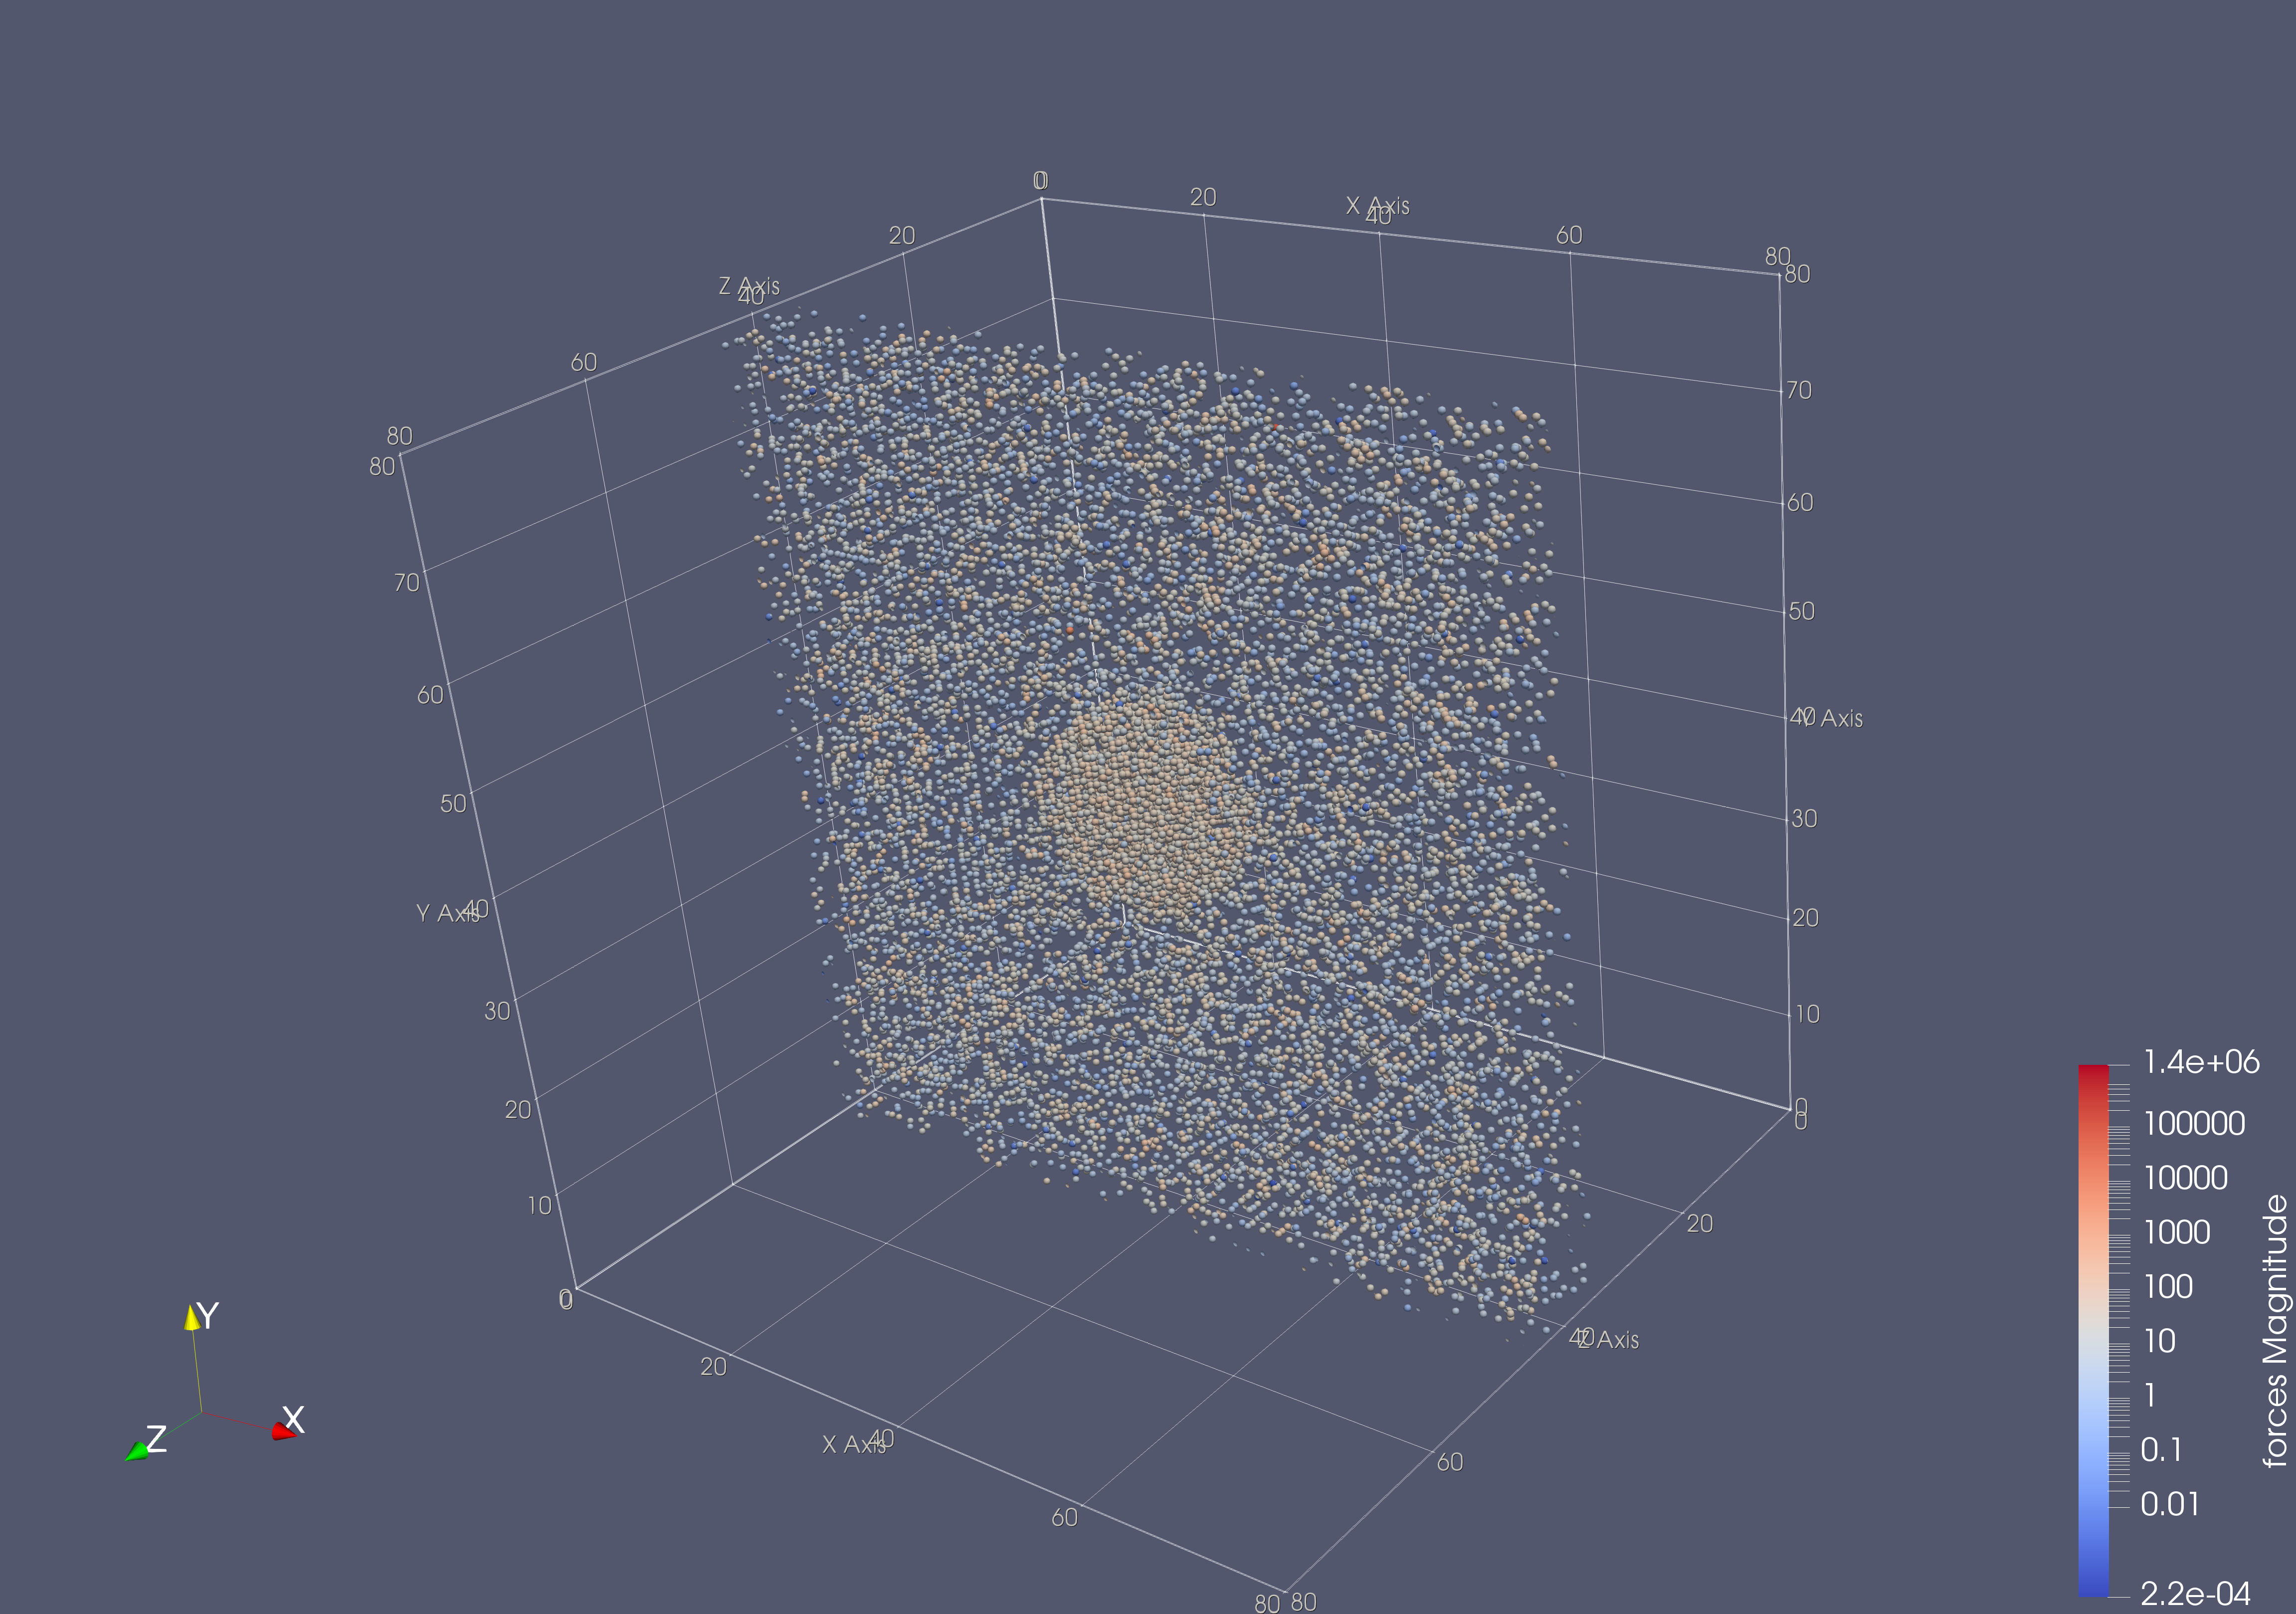
\includegraphics[width=.9\columnwidth]{figures/scenario_clip_rot.png}};
			\begin{scope}[x={(image.south east)},y={(image.north west)}]
				\draw[red, thin,rounded corners] (.42,.42) rectangle (.58,.6);
			\end{scope}
		\end{tikzpicture}
		\caption[Figure with tikz]{Figures can be drawn on or completely generated with tikz.}
		\label{fig:exampleLabel2}
	\end{figure}
\end{multicols}

\paragraph{Subfigures}
If grouping of several pictures seems reasonable, think about using subfigures. This often comes in handy with plots.

\begin{figure}[H]
	\centering
	\begin{subfigure}[b]{0.33\textwidth}
		\includegraphics[width=\textwidth]{example-image-a}
		\caption{example-image-a}
		\label{fig:example-image-a}
	\end{subfigure}
	\begin{subfigure}[b]{0.33\textwidth}
		\includegraphics[width=\textwidth]{example-image-b}
		\caption{example-image-b}
		\label{fig:example-image-b}
	\end{subfigure}
	\begin{subfigure}[b]{0.33\textwidth}
		\includegraphics[width=\textwidth]{example-image-c}
		\caption{example-image-c}
		\label{fig:example-image-c}
	\end{subfigure}
	\caption{One caption to describe them all.}
\end{figure}

\subsection{How to Algorithm}

\begin{figure}
	\begin{algorithm}[H]
		
		% Define custom keywords
		\SetKwFunction{KwNot}{not}
		% Define custom Functions
		\SetKwFunction{Fissorted}{is\_sorted}
		\SetKwFunction{Fbogosort}{bogosort}
		\SetKwFunction{Fshuffle}{shuffle}
		\SetKwProg{Fn}{Function}{:}{}
		\KwIn{\tabto{2cm}data array}
		\KwOut{\tabto{2cm} data sorted}
		\BlankLine
		
		\tcp{Checks if array is sorted}
		\Fn{\Fissorted{data}}{
			\For{i $\leftarrow$ 0 \KwTo data.size() - 1}{
				\label{algo:for}            % labels can also be put in the algorithm
				\If{data[i] $>$ data[i+1]}{
					\Return false
				}
			}
			\Return true
		}
		
		\tcp{actual algorithm}
		\Fn{\Fbogosort{data}}{
			\While{\KwNot \Fissorted{data}}{
				random.\Fshuffle{data}
			}
		}
		
		\caption[Bogosort]{Bogosort}
		\label{algo:example}
	\end{algorithm}
	\caption{some description what is happening}
\end{figure}

\clearpage

\subsection{How to Code}
\begin{lstlisting}[style=eclipse-cpp, caption=General form of a typical runner() function., label=code:runner]
	void runner(int type, void *data){
		switch(type)
		case taskType1:
		// do stuff using data
		case taskType2:
		// do other stuff using data
	}
\end{lstlisting}

\subsection{How to Table}
\begin{table}[H]
	\begin{tabularx}{\columnwidth}{L | C | R}
		\hline
		\hline
		bla left & bla centered\newline over two lines &  bla right\\
		\hline
		bla left & bla centered & \multirow[c]{2}{\hsize}{cell spanning two rows} \\
		\cline{1-2}
		\multicolumn{2}{c|}{cell spanning two columns} & \\
	\end{tabularx}
	\caption[Some Table]{Fancy table that can contain line breaks and extended cells.}
	\label{tab:example}
\end{table}

%TODO: Insert screenshots. Potentially even with the respective old version of a screen to see the development.

\listoffigures

\listoftables

\printbibliography

\printglossary[type=acronym,nonumberlist]

\printglossary[type=main,nonumberlist]

\end{document}
